\normaltrue \difficilefalse \tdifficilefalse
\correctiontrue
%\UPSTIidClasse{11} % 11 sup, 12 spé
%\newcommand{\UPSTIidClasse}{11}

\exer{Conception de la commande d’un robot chirurgical$\star$ \label{B2:07:78}}

% Concours Mines Ponts MP -- PSI --  2013

\setcounter{question}{0}\UPSTIcompetence[2]{B2-07}
\index{Compétence B2-07}
\index{Schéma-blocs}
\index{Robot}
\ifcorrection
\else
\marginnote{\textbf{Pas de corrigé pour cet exercice.}}
\fi




\ifprof
\else
\subsection*{Présentation du système}

Afin d’améliorer les conditions d’opérations chirurgicales dites mini invasives (comme la précision d’opération
et le confort du chirurgien), des robots chirurgicaux ont vu le jour. Cette étude s’intéresse à l’un d’entre eux : le
robot Da Vinci. Le chirurgien peut atteindre sa cible grâce à des outils longs et fins traversant le patient grâce
à une incision de l’ordre du centimètre.


Le système étudié est composé de deux sous-systèmes principaux :
\begin{itemize}
\item l’ensemble \{console de commande + bras maîtres\} permet au chirurgien de visualiser et de commander les
mouvements des outils adéquats à l’intérieur du patient via une caméra haute définition dont l’image est
retransmise par l’intermédiaire d’écrans. Le chirurgien commande les mouvements des outils grâce à deux
bras maîtres dont les extrémités sont maintenues dans chaque main ;
\item les bras esclaves reçoivent les consignes issues du chirurgien par l’intermédiaire des bras maîtres. Il y a au
total 3 bras esclaves : deux manipulent chacun un outil, le troisième manipule une caméra.
\end{itemize}
\begin{center}
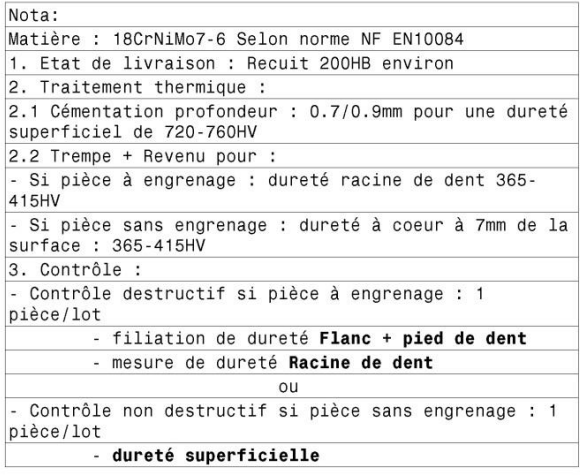
\includegraphics[width=\linewidth]{fig_02}
%\textit{}
\end{center}


Le mouvement de l'axe 1 est régi par l'équation suivante : 
$\Delta C_1(t)=J\dfrac{\dd^2 \Delta \theta_1(t)}{\dd t^2} - k_1 \dfrac{r_9'}{r_0}h_2 \Delta F_x(t)$ avec $J=\SI{1,98e-5}{kg.m^2}$, $k_1\dfrac{r_9'}{r_0}=0,00717$, $h_2=\SI{0,2}{m}$.

Le couple moteur $\Delta C_1(t)$ est fourni par une machine à courant continu modélisée par les équations suivantes : 
$u_1(t)=L\dfrac{\dd i_1(t)}{\dd t}  + Ri_1(t)+e_1(t)$, $e_1(t)=k_e \dfrac{\dd \Delta \theta_1(t)}{\dd t}$, $\Delta C_1(t) = k_t i_1(t)$ avec $u_1(t)$ la tension aux bornes du moteur, $i_1(t)$ l’intensité traversant le moteur et $e_1(t)$ la force contre
électromotrice, avec $R=\SI{2,08}{\Omega}$, $k_t = \SI{0,0525}{N.m.A^{-1}}$ et $k_e = \SI{0,0525}{V.s.rad^{-1}}$.

On fait l’hypothèse que l’influence de l’inductance $L$ est négligeable sur les performances attendues, soit $L=0$.

La consigne est notée $\Delta \theta _{c1}(t)$. Le cahier des charges sélectif conduit à choisir un correcteur associant une anticipation (via la présence de $\sigma_4$ dans la relation suivante) et une correction PID. La tension de commande du moteur est donnée par : $U_1(p)=\left( \Delta \theta_{c1}(p)-\Delta \theta_1(p)\right) \left(\sigma_1 + \dfrac{\sigma_2}{p}\right)- \sigma_3p \Delta \theta_1(p)+\sigma_4\Delta \theta_{c1}(p)$
avec $\Delta \theta_{c1}(p)$ la consigne de position angulaire exprimée dans le domaine symbolique.
\fi


\question{Compléter le schéma-blocs.}
\ifprof
\begin{corrige} ~\\

\begin{center}
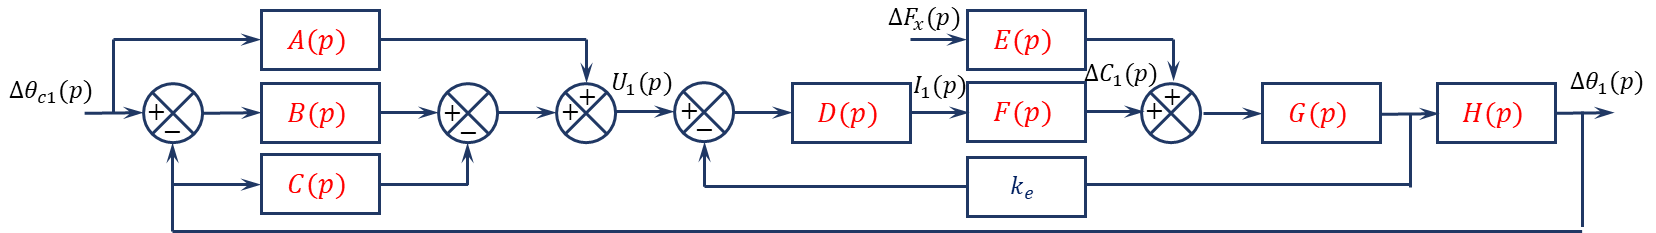
\includegraphics[width=\linewidth]{cor_02}
%\textit{}
\end{center}


En utilisant l'équation électrique du MCC, on a 
$U_1(p)=\left(L p   + R\right)I_1(p)+E_1(p)$. En utilisant le schéma-blocs :  $I_1(p)=\left(U_1(p) - E(p)\right) D(p)$. On a donc 
$I_1(p)=\dfrac{U_1(p) - E(p)}{R+Lp}$ et $D(p) = \dfrac{1}{R+Lp}$.

En utilisant la première relation de comportement du MCC, on a $E_1(p)$ en sortie du bloc $k_e$ et $p\Delta_1(p)$ en entrée; donc $H(p)=\dfrac{1}{p}$.

En utilisant la seconde relation, on a $F(p)=k_t$.

En utilisant l'équation de mouvement de l'axe 1, on a :
$\Delta C_1(p)=J p ^2  \Delta \theta_1(p) - k_1 \dfrac{r_9'}{r_0}h_2 \Delta F_x(p)$.

D'après le schéma-blocs, on a $\Delta \theta_1(p) = \left(\Delta C_1(p)+\Delta F_x(p) E(p)\right) G(p)H(p)$.

En réageançant l'équation, on a 
$J p ^2  \Delta \theta_1(p) = \Delta C_1(p) +  k_1 \dfrac{r_9'}{r_0}h_2 \Delta F_x(p) $
$ \Leftrightarrow   \Delta \theta_1(p) = \left(\Delta C_1(p) +  k_1 \dfrac{r_9'}{r_0}h_2 \Delta F_x(p)\right) \dfrac{1}{J p ^2} $.

On a donc $E(p)= k_1 \dfrac{r_9'}{r_0}h_2 $. 

De plus $G(p)H(p)=\dfrac{1}{Jp^2}$ et $H(p)=\dfrac{1}{p}$; donc $G(p)=\dfrac{1}{Jp}$.


En utilisant l'équation électrique du MCC, on a 
$U_1(p)=\left(L p   + R\right)I_1(p)+E_1(p)$. En utilisant le schéma-blocs :  $I_1(p)=\left(U_1(p) - E(p)\right) D(p)$. On a donc 
$I_1(p)=\dfrac{U_1(p) - E(p)}{R+Lp}$ et $D(p) = \dfrac{1}{R+Lp}$.


En utilisant l'équation du PID, on a 
$U_1(p)=\left( \Delta \theta_{c1}(p)-\Delta \theta_1(p)\right) \left(\sigma_1 + \dfrac{\sigma_2}{p}\right)- \sigma_3p \Delta \theta_1(p)+\sigma_4\Delta \theta_{c1}(p)$
soit $U_1(p)=\left( \Delta \theta_{c1}(p) \left(\sigma_1 + \dfrac{\sigma_2}{p}\right) -\Delta \theta_1(p) \left(\sigma_1 + \dfrac{\sigma_2}{p}\right)\right) - \sigma_3p \Delta \theta_1(p)+\sigma_4\Delta \theta_{c1}(p)$.

En utilisant le schéma-blocs, on a 
$U_1(p)=\Delta_{c1}(p) A(p) + \left(\Delta_{c1}(p) -\Delta\theta_{1}(p)\right) B(p) - \Delta\theta_{1}(p)C(p)$
$=\Delta_{c1}(p) \left( A(p) + B(p)\right) -\Delta\theta_{1}(p)  \left(B(p)+C(p)\right)$.

Par suite, 
$U_1(p)= \Delta \theta_{c1}(p) \left(\sigma_1 + \dfrac{\sigma_2}{p} +\sigma_4\right) -\Delta \theta_1(p) \left(\sigma_1 + \dfrac{\sigma_2}{p} + \sigma_3p\right)$.

On aura donc $B(p)=\sigma_1 + \dfrac{\sigma_2}{p}$, $C(p)=\sigma_3 p$ et  $A(p)=\sigma_4$.


\begin{center}
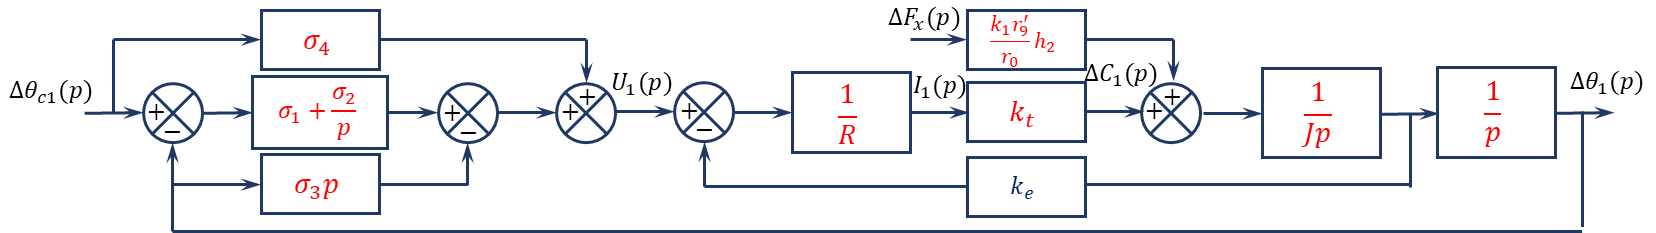
\includegraphics[width=\linewidth]{cor_03}
%\textit{}
\end{center}
\end{corrige}
\else
\fi


\ifprof
\else
Pour la suite, on considère la perturbation nulle ($\Delta F_x(p)=0$).
\fi

\question{À partir de ce schéma-blocs, en notant $H_{\text{processus}}(p)=\dfrac{\Delta \theta_1(p)}{U_1(p)}=\dfrac{K}{p\left(1+\tau p \right)}$, exprimer $K$ et $\tau$ en fonction des données de l'énoncé.}
\ifprof
\begin{corrige}
On a $H_{\text{processus}}(p)= \dfrac{D(p)F(p)G(p)}{1+D(p)F(p)G(p) k_e} H(p)$
soit $H_{\text{processus}}(p)= \dfrac{\dfrac{1}{R+Lp}k_t\dfrac{1}{Jp}}{1+\dfrac{1}{R+Lp}k_t\dfrac{1}{Jp} k_e} \dfrac{1}{p}$.
Avec $L=0$, 
$H_{\text{processus}}(p) =\dfrac{k_t}{RJp+k_t k_e} \dfrac{1}{p}=\dfrac{\dfrac{1}{k_e}}{\dfrac{RJ}{k_t k_e}p+1} \dfrac{1}{p}$ soit $K = \dfrac{1}{k_e}$ et $\tau = \dfrac{RJ}{k_t k_e}$.
\end{corrige}
\else
\fi



\question{Exprimer la fonction de transfert en boucle fermée, sous sa forme canonique, notée $B_F(p) = \dfrac{\Delta \theta_1(p)}{\Delta \theta_{c1}(p)}$ en fonction de $K$, $\tau$, $\sigma_1$, $\sigma_2$, $\sigma_3$ et  $\sigma_4$.}
\ifprof
\begin{corrige}
On a vu que $U_1(p)= \Delta \theta_{c1}(p) \left(\sigma_1 + \dfrac{\sigma_2}{p} +\sigma_4\right) -\Delta \theta_1(p) \left(\sigma_1 + \dfrac{\sigma_2}{p} + \sigma_3p\right)$ et 
que $\dfrac{\Delta \theta_1(p)}{U_1(p)}=\dfrac{K}{p\left(1+\tau p \right)}$.

On a donc 
$\Delta \theta_1(p) \dfrac{p\left(1+\tau p \right)}{K}= \Delta \theta_{c1}(p) \left(\sigma_1 + \dfrac{\sigma_2}{p} +\sigma_4\right) -\Delta \theta_1(p) \left(\sigma_1 + \dfrac{\sigma_2}{p} + \sigma_3p\right)$

$\Leftrightarrow \Delta \theta_1(p) \left(\dfrac{p\left(1+\tau p \right)}{K}  + \sigma_1 + \dfrac{\sigma_2}{p} + \sigma_3p\right)= \Delta \theta_{c1}(p) \left(\sigma_1 + \dfrac{\sigma_2}{p} +\sigma_4\right) $ et 

$B_F(p) = \dfrac{\sigma_1 + \dfrac{\sigma_2}{p} +\sigma_4}{\dfrac{p\left(1+\tau p \right)}{K}  + \sigma_1 + \dfrac{\sigma_2}{p} + \sigma_3p}$ 
$= \dfrac{\sigma_1 p + \sigma_2 + \sigma_4 p}{\dfrac{p^2\left(1+\tau p \right)}{K}  + \sigma_1p + \sigma_2 + \sigma_3p^2}$
$= K \dfrac{\sigma_1 p + \sigma_2 + \sigma_4 p}{p^2\left(1+\tau p \right)  + \sigma_1 K p + \sigma_2 K  + \sigma_3 Kp^2}$
$= K \dfrac{\left(\sigma_1+ \sigma_4 \right) p + \sigma_2 }{ \tau p^3 + p^2\left(1+\sigma_3 \right)  + \sigma_1 K p + \sigma_2 K  }$.
\end{corrige}
\else
\fi



\ifprof
\else
\begin{center}
\rotatebox{90}{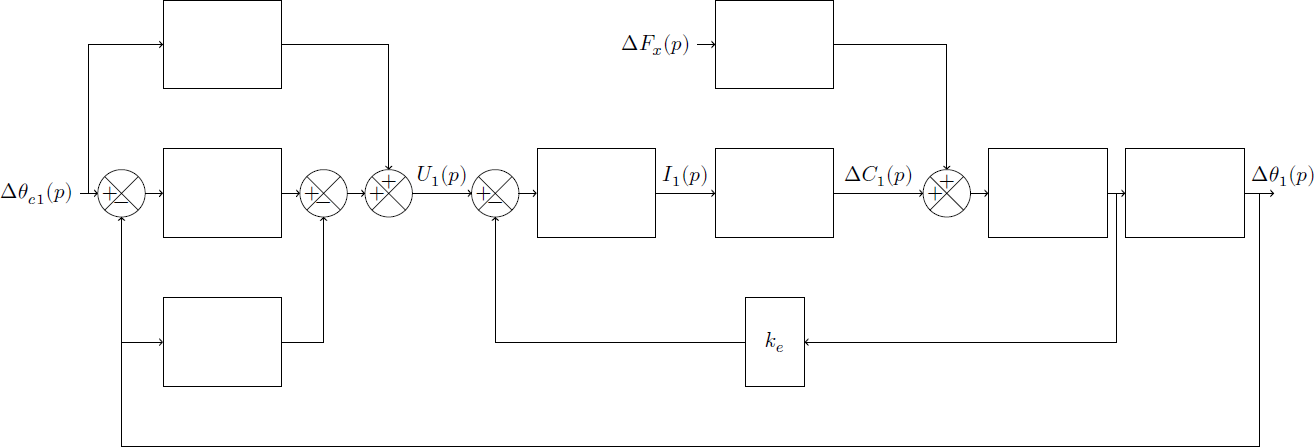
\includegraphics[height=.9\linewidth]{fig_03}}
%\textit{Schéma-blocs de l'asservissement du dosseret \label{fig6}}
\end{center}
\fi


\ifprof
\else
\footnotesize
\begin{tabular}{|p{.95\linewidth}|}
\hline
\begin{enumerate}
\item 
$A(p)=\sigma_4$,
$B(p)=\sigma_1 + \dfrac{\sigma_2}{p}$, 
$C(p)=\sigma_3 p$, 
$D(p) = \dfrac{1}{R+Lp}$, 
$E(p)= k_1 \dfrac{r_9'}{r_0}h_2 $, 
$F(p)=k_t$, 
$G(p)=\dfrac{1}{Jp}$, 
$H(p)=\dfrac{1}{p}$.
\item $K = \dfrac{1}{k_e}$ et $\tau = \dfrac{RJ}{k_t k_e}$.
\item $B_F(p) = K \dfrac{\left(\sigma_1+ \sigma_4 \right) p + \sigma_2 }{ \tau p^3 + p^2\left(1+\sigma_3 \right)  + \sigma_1 K p + \sigma_2 K  }$.
\end{enumerate} \\
\hline
\end{tabular}
\normalsize
\begin{flushright}
\footnotesize{Corrigé  voir \ref{B2:07:78}.}
\end{flushright}%
\fi